\item Wir betrachten ein Polynom der Form $p(x) = a\cdot \left(x-x_0\right)^n+k$.

\begin{multicols}{2}
  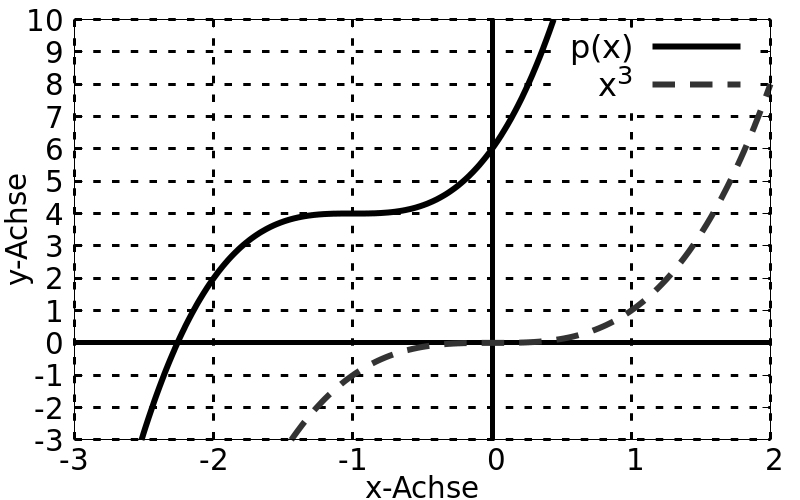
\includegraphics[width=0.45\textwidth]{../gnuplot/ex-fn-transform-2-a.png}

\begin{enumerate}
\item Welchen Grad hat das Polynom? Wie lautet der höchste Koeffizient?
\item Wie ist $p$ relativ zu $f(x)=x^3$ verschoben und skaliert? (Reihenfolge der Transformationen beachten!)
\item Finden Sie eine Funkionsgleichung für den Graphen $p(x)$ in der nebenstehenden Skizze! 
\item Finden Sie eine Funktionsgleichung für eine nach oben geöffnete Parabel, sodass der Scheitelpunkt bei $(1,3)$ liegt; und jeweils 1 Einheit links und rechts vom Scheitelpunkt der Funktionswert um 4 Einheiten größer ist als am Scheitelpunkt.
\item Ermitteln Sie $a$, $x_0$, $n$ und $k$ für $p(x)=4x^2-7x+3$, indem Sie die Gleichung $a\cdot \left(x-x_0\right)^n+k = 4x^2-7x+3$ mittels Koeffizientenvergleich lösen!
\end{enumerate}

\end{multicols}

